\documentclass[12pt]{article}\usepackage[]{graphicx}\usepackage[]{color}
%% maxwidth is the original width if it is less than linewidth
%% otherwise use linewidth (to make sure the graphics do not exceed the margin)
\makeatletter
\def\maxwidth{ %
  \ifdim\Gin@nat@width>\linewidth
    \linewidth
  \else
    \Gin@nat@width
  \fi
}
\makeatother

\definecolor{fgcolor}{rgb}{0.345, 0.345, 0.345}
\newcommand{\hlnum}[1]{\textcolor[rgb]{0.686,0.059,0.569}{#1}}%
\newcommand{\hlstr}[1]{\textcolor[rgb]{0.192,0.494,0.8}{#1}}%
\newcommand{\hlcom}[1]{\textcolor[rgb]{0.678,0.584,0.686}{\textit{#1}}}%
\newcommand{\hlopt}[1]{\textcolor[rgb]{0,0,0}{#1}}%
\newcommand{\hlstd}[1]{\textcolor[rgb]{0.345,0.345,0.345}{#1}}%
\newcommand{\hlkwa}[1]{\textcolor[rgb]{0.161,0.373,0.58}{\textbf{#1}}}%
\newcommand{\hlkwb}[1]{\textcolor[rgb]{0.69,0.353,0.396}{#1}}%
\newcommand{\hlkwc}[1]{\textcolor[rgb]{0.333,0.667,0.333}{#1}}%
\newcommand{\hlkwd}[1]{\textcolor[rgb]{0.737,0.353,0.396}{\textbf{#1}}}%

\usepackage{framed}
\makeatletter
\newenvironment{kframe}{%
 \def\at@end@of@kframe{}%
 \ifinner\ifhmode%
  \def\at@end@of@kframe{\end{minipage}}%
  \begin{minipage}{\columnwidth}%
 \fi\fi%
 \def\FrameCommand##1{\hskip\@totalleftmargin \hskip-\fboxsep
 \colorbox{shadecolor}{##1}\hskip-\fboxsep
     % There is no \\@totalrightmargin, so:
     \hskip-\linewidth \hskip-\@totalleftmargin \hskip\columnwidth}%
 \MakeFramed {\advance\hsize-\width
   \@totalleftmargin\z@ \linewidth\hsize
   \@setminipage}}%
 {\par\unskip\endMakeFramed%
 \at@end@of@kframe}
\makeatother

\definecolor{shadecolor}{rgb}{.97, .97, .97}
\definecolor{messagecolor}{rgb}{0, 0, 0}
\definecolor{warningcolor}{rgb}{1, 0, 1}
\definecolor{errorcolor}{rgb}{1, 0, 0}
\newenvironment{knitrout}{}{} % an empty environment to be redefined in TeX

\usepackage{alltt}
\usepackage{amsmath}
\usepackage{amsthm}
\usepackage{graphicx,psfrag,epsf}
\usepackage{enumerate}
\usepackage{booktabs}
\RequirePackage[natbibapa]{apacite}
\usepackage{caption}
\usepackage{multirow}

% NOTE: To produce blinded version, replace "0" with "1" below.
\newcommand{\blind}{0}

% DON'T change margins - should be 1 inch all around.
\addtolength{\oddsidemargin}{-.5in}%
\addtolength{\evensidemargin}{-.5in}%
\addtolength{\textwidth}{1in}%
\addtolength{\textheight}{1.3in}%
\addtolength{\topmargin}{-.8in}%

\usepackage{float}    % for fig.pos='H'
\usepackage{rotfloat} % for sidewaysfigure

\usepackage[textwidth=1in, textsize=tiny]{todonotes}

\newtheorem{thm}{Theorem}
\newtheorem{lem}{Lemma}

\newcommand{\Prob}{\text{Pr}}
\newcommand{\E}{\text{E}}
\newcommand{\Cov}{\text{Cov}}
\newcommand{\corr}{\text{corr}}
\newcommand{\Var}{\text{Var}}
\newcommand{\iid}{\stackrel{\text{iid}}{\sim}}
\newcommand{\tr}{\text{tr}}
\newcommand{\bm}{\mathbf}
\newcommand{\bs}{\boldsymbol}
\IfFileExists{upquote.sty}{\usepackage{upquote}}{}
\begin{document}
\def\spacingset#1{\renewcommand{\baselinestretch}%
{#1}\small\normalsize} \spacingset{1}


%%%%%%%%%%%%%%%%%%%%%%%%%%%%%%%%%%%%%%%%%%%%%%%%%%%%%%%%%%%%%%%%%%%%%%%%%%%%%%

\if0\blind
{
  \title{\bf Small sample methods for cluster-robust variance estimation and hypothesis testing in fixed effects models\thanks{The authors thank Dan Knopf for helpful discussions about the linear algebra behind the cluster-robust variance estimator.}}
  \author{\\James E. Pustejovsky\thanks{Department of Educational Psychology, University of Texas at Austin, 1912 Speedway, Stop D5800, Austin, TX 78712. Email: pusto@austin.utexas.edu}
    \hspace{.2cm}and\hspace{.2cm}
    Elizabeth Tipton\thanks{Department of Human Development, Teachers College, Columbia University, 425 W. 120th Street
New York, NY, USA 10027. Email: tipton@tc.columbia.edu}
    }
  \maketitle
} \fi

\if1\blind
{
  \bigskip
  \bigskip
  \bigskip
  \begin{center}
    {\LARGE\bf Small sample methods for cluster-robust variance estimation and hypothesis testing in fixed effects models}
\end{center}
  \medskip
} \fi

\bigskip


\begin{abstract}
In panel data models and other regressions with unobserved effects, fixed effects estimation is often paired with cluster-robust variance estimation (CRVE) in order to account for heteroskedasticity and un-modeled dependence among the errors. 
Although asymptotically consist, CRVE can be biased downward when the number of clusters is small, leading to hypothesis tests with rejection rates that are too high. 
More accurate tests can be constructed using bias-reduced linearization (BRL), which corrects the CRVE based on a working model, in conjunction with a Satterthwaite approximation for t-tests. 
We propose a generalization of BRL that can be applied in models with arbitrary sets of fixed effects, where the original BRL method is undefined, and describe how to apply the method when the regression is estimated after absorbing the fixed effects. 
We also propose a small-sample test for multiple-parameter hypotheses, which generalizes the Satterthwaite approximation for t-tests. 
In simulations covering a wide range of scenarios, we find that conventional cluster-robust Wald tests can severely over-reject while the proposed small-sample test maintains Type I error close to nominal levels. 
An R package implementing the proposed methods is available on the Comprehensive R Archive Network. 
\end{abstract}

\noindent%
{\it Keywords:} cluster dependence, fixed effects, robust standard errors, small samples
\vfill

\newpage
\spacingset{1.45} % DON'T change the spacing!


\section{INTRODUCTION}
\label{sec:intro}

In many economic analyses, interest centers on the parameters of a linear regression model, estimated by ordinary or weighted least squares (OLS/WLS) from data exhibiting within-group dependence. 
Such dependence can arise from sampling of aggregate units (e.g., counties, districts, villages), each of which contains multiple observations; from repeated measurement of an outcome on a common set of units, as in panel data; or from model misspecification, as in analysis of regression discontinuity designs \citep[e.g.,][]{Lee2008regression}. 
A common approach to inference in these settings is to use a cluster-robust variance estimator \citep[CRVE;][]{Arellano1987computing, Liang1986longitudinal, white1984asymptotic}.
The advantage of the CRVE is that it produces consistent standard errors and test statistics without imposing strong parametric assumptions about the correlation structure of the errors in the model.
Instead, the method relies on the weaker assumption that units can be grouped into clusters that are mutually independent. 
%CRVE is an extension to another economic mainstay, heteroskedasticity-consistent variance estimators \citep{Huber1967behavior, White1980heteroskedasticity}, which are used to account for non-constant variance in regression models with uncorrelated errors.
In the past decade, use of CRVEs has become standard practice for micro-economic researchers, as evidenced by coverage in major textbooks and review articles \citep[e.g.,][]{Wooldridge2010econometric, Angrist2009mostly, Cameron2015practitioners}.

As a leading example, consider a difference-in-differences analysis of state-by-year panel data, where the goal is to understand the effects on employment outcomes of several state-level policy shifts. 
Each policy effect would be parameterized as a dummy variable in a regression model, which might also include other demographic controls. It is also common to include fixed effects for each state and each time-point in order to control for unobserved confounding in each dimension. 
The model could be estimated by least squares with the fixed effects included as dummy variables (or what we will call the LSDV estimator). More commonly, the effects of the policy indicators would be estimated after absorbing the fixed effects, a computational technique that is also known as the fixed effects estimator or ``within transformation'' \citep{Wooldridge2010econometric}. 
Standard errors would then be clustered by state to account for residual dependence in the errors from a given state, and these clustered standard errors would be used to test hypotheses about the set of policies.
The need to cluster the standard errors by state, even when including state fixed effects, was highlighted by \citet{Bertrand2004how}, who showed that to do otherwise can lead to inappropriately small standard errors and hypothesis tests with incorrect rejection rates. 

The consistency property of CRVEs is asymptotic in the number of independent clusters \citep{Wooldridge2003cluster}.
Recent methodological work has demonstrated that CRVEs can be biased downward and associated hypothesis tests can have Type-I error rates considerably in excess of nominal levels when based on a small or moderate number of clusters \citep[e.g.,][]{MacKinnon2016wild}.
\citet{Cameron2015practitioners} provide an extensive review of this literature, including a discussion of current practice, possible solutions, and open problems. 
In particular, they demonstrate that small-sample corrections for t-tests implemented in common software packages such as Stata and SAS do not provide adequate control of Type-I error. 

\citet{Bell2002bias} proposed a method that improves the small-sample properties of CRVEs \citep[see also][]{McCaffrey2001generalizations}. 
Their method, called bias-reduced linearization (BRL), entails adjusting the CRVE so that it is exactly unbiased under a working model specified by the analyst, while also remaining asymptotically consistent under arbitrary true variance structures. 
Simulations reported by \citet{Bell2002bias} demonstrate that the BRL correction serves to reduce the bias of the CRVE even when the working model is misspecified. 
The same authors also proposed and studied small-sample corrections to single-parameter hypothesis tests using the BRL variance estimator, based on Satterthwaite \citep{Bell2002bias} or saddlepoint approximations \citep{McCaffrey2006improved}. 
In an analysis of a longitudinal cluster-randomized trial with 35 clusters, \citet{Angrist2009effects} observed that the BRL correction makes a difference for inferences. 

Despite a growing body of evidence that BRL performs well \citep[e.g.,][]{Imbens2015robust}, several problems with the method hinder its wider application. 
First, \citet{Angrist2009mostly} noted that the BRL correction is undefined in some highly parameterized models, such as state-by-year panels that include fixed effects for states and for years \citep[see also][]{Young2016improved}.
Second, in models with fixed effects, the magnitude of the BRL adjustment depends on whether it is computed based on the full design matrix (i.e., the LSDV estimator) or after absorbing the fixed effects.  
Third, extant methods for hypothesis testing based on BRL are limited to single-parameter constraints \citep{Bell2002bias, McCaffrey2006improved} and small-sample methods for multiple-parameter hypothesis tests remain lacking.
%Multiple-parameter tests are used in a range of applications, including in panel data settings (e.g., Hausman tests for consistency of random effects estimators), seemingly unrelated regression models, and analysis of field experiments with multiple treatment groups.

This paper addresses each of these concerns in turn, with the aim of extending the BRL method so that is suitable for general application. 
First, we describe a simple modification of the BRL adjustment that remains well-defined in models with arbitrary sets of fixed effects, where existing BRL adjustments break down. 
Second, we demonstrate how to calculate the BRL adjustments based on the fixed effects estimator and identify conditions under which first-stage absorption of the fixed effects can be ignored.
Finally, we propose a procedure for testing multiple-parameter hypotheses by approximating the sampling distribution of the Wald statistic using Hotelling's $T^2$ distribution with estimated degrees of freedom. 
The method is a generalization of the Satterthwaite correction proposed by \citet{Bell2002bias} for single parameter constraints. 
The proposed methods are implemented in an R package, available on the Comprehensive R Archive Network.\todo{Cite package clubSandwich.} 

Our work is related to a stream of recent literature that has examined methods for cluster-robust inference with a small number of clusters. 
\citet{Conley2011inference} proposed methods for hypothesis testing in a difference-in-differences setting where the number of treated units is small and fixed, while the number of untreated units increases asymptotically. 
\citet{Ibragimov2010tstatistic} proposed a cluster-robust t-test that maintains the nominal Type-I error rate; however, their method requires that the target parameter be identified within each independent cluster and so it is not always applicable.
\citet{Young2016improved} proposed a Satterthwaite correction for t-tests based on a different type of bias correction to the CRVE, where the bias correction term is derived under a working model.
\citet{Cameron2008bootstrap} investigated a range of bootstrapping procedures that provide improved Type-I error control in small samples, finding that a cluster wild-bootstrap technique was particularly accurate in small samples. 
Nearly all of this work has focused on single-parameter hypothesis tests only. 
For multiple-parameter constraints, \citet{Cameron2015practitioners} suggested an ad hoc degrees of freedom adjustment and noted, as an alternative, that bootstrapping techniques can in principle be applied to multiple-parameter tests. 
However, little methodological work has examined the accuracy of multiple-parameter tests.

The paper is organized as follows. The remainder of this section introduces our econometric framework and reviews the standard CRVE methods, as implemented in most software applications.
Section \ref{sec:BRL} reviews the original BRL correction and describes modifications that make it possible to implement BRL in a broad class of models with fixed effects.
Section \ref{sec:testing} discusses hypothesis tests based on the BRL-adjusted CRVE. 
Section \ref{sec:simulation} reports a simulation study examining the null rejection rates of multiple-parameter hypothesis tests, where we find that the small-sample test offers drastic improvements over commonly implemented alternatives. 
Section \ref{sec:examples} illustrates the use of the proposed hypothesis tests in two applications. 
Section \ref{sec:conclusion} concludes and discusses avenues for future work. 

\subsection{Econometric framework}

We consider a linear regression model of the form,
\begin{equation}
\label{eq:fixed_effects}
\bm{y}_i = \bm{R}_i \bs\beta + \bm{S}_i \bs\gamma + \bm{T}_i \bs\mu + \bs\epsilon_i,
\end{equation}
where $\bm{y}_i$ is a vector of $n_i$ outcomes for cluster $i$,  $\bm{R}_i$ is an $n_i \times r$ matrix containing predictors of primary interest (e.g., policy variables) and any additional controls, $\bm{S}_i$ is an $n_i \times s$ matrix describing fixed effects that vary across clusters, and $\bm{T}_i$ is an $n_i \times t$ matrix describing cluster-specific fixed effects, which must satisfy $\bm{T}_h \bm{T}_i' = \bm{0}$ for $h \neq i$.
Note that the distinction between the covariates $\bm{R}_i$ versus the fixed effects $\bm{S}_i$ is arbitrary and depends on the analyst's inferential goals.
In a fixed effects model for state-by-year panel data, $\bm{R}_i$ would include indicator variables for policy changes, as well as additional demographic controls; $\bm{S}_i$ would include year fixed effects; and $\bm{T}_i$ would indicate state fixed effects (or perhaps also state-specific time trends). 
Interest would center on testing hypotheses regarding the coefficients in $\bs\beta$ that correspond to the policy indicators, while $\bs\gamma$ and $\bs\mu$ would be treated as incidental. 

We shall assume that $\E\left(\bs\epsilon_i\left|\bm{R}_i,\bm{S}_i, \bm{T}_i\right.\right) = \bm{0}$ and $\Var\left(\bs\epsilon_i\left|\bm{R}_i,\bm{S}_i,\bm{T}_i\right.\right) = \bs\Sigma_i$, for $i = 1,...,m$, where the form of $\bs\Sigma_1,...,\bs\Sigma_m$ may be unknown but the errors are independent across clusters. 
Let $\bm{U}_i = \left[\bm{R}_i \ \bm{S}_i \right]$ denote the set of predictors that vary across clusters\todo{Clarify this?}, $\bm{X}_i = \left[\bm{R}_i \ \bm{S}_i \ \bm{T}_i \right]$ denote the full set of predictors, $\bs\alpha = \left(\bs\beta', \bs\gamma', \bs\mu' \right)'$, and $p = r + s + t$.
Let $N = \sum_{i=1}^m n_i$ denote the total number of observations.
Let $\bm{y}$, $\bm{R}$, $\bm{S}$, $\bm{T}$, $\bm{U}$, $\bm{X}$, and $\bs\epsilon$ denote the matrices obtained by stacking their corresponding components, as in $\bm{R} = \left(\bm{R}_1' \ \bm{R}_2' \ \cdots \ \bm{R}_m'\right)'$. 

We assume that $\bs\beta$ is estimated by weighted least squares (WLS) using symmetric, full rank weighting matrices $\bm{W}_1,...,\bm{W}_m$. 
Clearly, the WLS estimator includes OLS as a special case.
More generally, the WLS estimator encompasses feasible GLS, where it is assumed that $\Var\left(\bm{e}_i\left|\bm{X}_i\right.\right) = \bs\Phi_i$, a known function of a low-dimensional parameter. 
For example, an auto-regressive error structure might be posited to describe repeated measures on an individual over time. 
The weighting matrices are then taken to be $\bm{W}_i = \hat{\bs\Phi}_i^{-1}$, where the $\hat{\bs\Phi}_i$ are constructed from estimates of the variance parameter.
Finally, for analysis of data from complex survey designs, WLS may be used with sampling weights in order to account for unequal selection probabilities.

\subsection{Absorption}

The goal of most analyses is to estimate and test hypotheses regarding the parameters in $\bs\beta$, while the fixed effects $\bs\gamma$ and $\bs\mu$ are not of inferential interest. Furthermore, LSDV estimation becomes computationally intensive and numerically inaccurate if the model includes a large number of fixed effects (i.e., $s + t$ large). 
A commonly implemented alternative to LSDV is to first absorb the fixed effects, which leaves only the $r$ parameters in $\bs\beta$ to be estimated. 
Because Section \ref{sec:BRL} examines the implications of absorption for application of the BRL adjustment, we now formalize the absorption procedure.
Denote the full block-diagonal weighting matrix as $\bm{W} = \text{diag}\left(\bm{W}_1,...,\bm{W}_m\right)$.
Let $\bm{K}$ be the $x \times r$ matrix that selects the covariates of interest, so that $\bm{X} \bm{K} = \bm{R}$ and $\bm{K}'\bs\alpha = \bs\beta$.
For a generic matrix $\bm{Z}$ of full column rank, let $\bm{M_Z} = \left(\bm{Z}'\bm{W}\bm{Z}\right)^{-1}$ and $\bm{H_Z} = \bm{Z}\bm{M_Z}\bm{Z}'\bm{W}$. 

The absorption technique involves obtaining the residuals from the regression of $\bm{y}$ on $\bm{T}$ and from the multivariate regressions of $[\bm{R}$ and $\bm{S}]$ on $\bm{T}$. 
The $\bm{y}$ residuals and $\bm{R}$ residuals are then regressed on the $\bm{S}$ residuals. 
Finally, these twice-regressed $\bm{y}$ residuals are regressed on the twice-regressed $\bm{R}$ residuals to obtain the WLS estimates of $\bs\beta$. 
Let $\bm{\ddot{S}} = \left(\bm{I} - \bm{H_T}\right)\bm{S}$, $\bm{\ddot{R}} = \left(\bm{I} - \bm{H_{\ddot{S}}}\right)\left(\bm{I} - \bm{H_T}\right)\bm{R}$, and $\bm{\ddot{y}} = \left(\bm{I} - \bm{H_{\ddot{S}}}\right)\left(\bm{I} - \bm{H_T}\right)\bm{y}$. 
In what follows, subscripts on $\bm{\ddot{R}}$, $\bm{\ddot{S}}$,  $\bm{\ddot{U}}$, and $\bm{\ddot{y}}$ refer to the rows of these matrices corresponding to a specific cluster. 
The WLS estimator of $\bs\beta$ can then be written as
\begin{equation}
\label{eq:WLS}
\bs{\hat\beta} = \bm{M_{\ddot{R}}} \sum_{i=1}^m \bm{\ddot{R}}_i' \bm{W}_i \bm{\ddot{y}}_i. 
\end{equation}
This estimator is algebraically identical to the LSDV estimator, $\bs{\hat\beta} = \bm{K}'\bm{M_X} \bm{X}' \bm{W} \bm{y}$, but avoids the need to solve a system of $p$ linear equations. In the remainder, we assume that fixed effects are absorbed before estimation of $\bs\beta$. 
%For models that do not include within-cluster fixed effects, so that the full covariate matrix is $\bm{U} = \left[\bm{R} \ \bm{S}\right]$, all of the results hold after substituting $\bm{U}$ for $\bm{\ddot{R}}$. 

\subsection{Standard CRVE}

The WLS estimator $\bs{\hat\beta}$, has true variance
\begin{equation}
\label{eq:var_WLS}
\Var\left(\bs{\hat\beta}\right) = \bm{M_{\ddot{R}}}\left(\sum_{i=1}^m \bm{\ddot{R}}_i' \bm{W}_i \bs\Sigma_i \bm{W}_i\bm{\ddot{R}}_i\right) \bm{M_{\ddot{R}}},
\end{equation}
which depends upon the unknown variance matrices $\bs\Sigma_i$. 
%A model-based approach to estimating this variance would involve assuming that $\bm\Sigma_i$ follows a structure defined by some low-dimensional parameter; for example, it may be assumed that the structure was hierarchical or auto-regressive. 
%The model-based variance estimator would substitute estimates of $\bs\Sigma_i$ into (\ref{eq:var_WLS}).
%However, if the model is misspecified, this estimator will be inconsistent and inferences based upon it will be invalid.
The CRVE involves estimating $\Var\left(\bs{\hat\beta}\right)$ empirically, without imposing structural assumptions on $\bs\Sigma_i$. 
There are several versions of this approach, all of which can be written as
\begin{equation}
\label{eq:V_small}
\bm{V}^{CR} = \bm{M_{\ddot{R}}}\left(\sum_{i=1}^m \bm{\ddot{R}}_i'\bm{W}_i \bm{A}_i \bm{e}_i \bm{e}_i' \bm{A}_i' \bm{W}_i \bm{\ddot{R}}_i\right) \bm{M_{\ddot{R}}},
\end{equation}
where $\bm{e}_i = \bm{Y}_i - \bm{X}_i \bs{\hat\beta}$ is the vector of residuals from cluster $i$ and $\bm{A}_i$ is some $n_i$ by $n_i$ adjustment matrix. 

The form of the adjustment matrices parallels those of the heteroskedasticity-consistent variance estimators proposed by \citet*{MacKinnon1985some}. 
The original and most basic CRVE, described by \citet{Liang1986longitudinal}, uses $\bm{A}_i = \bm{I}_i$, an $n_i \times n_i$ identity matrix. 
Following \citet{Cameron2015practitioners}, we refer to this estimator as CR0. 
This estimator is biased towards zero because the cross-product of the residuals $\bm{e}_i \bm{e}_i'$ tends to under-estimate the true variance $\bs\Sigma_i$ in cluster $i$.
A rough bias adjustment is to take $\bm{A}_i = c\bm{I}_i$, where $c = \sqrt{(m/(m-1))}$; we denote this adjusted estimator as CR1. Some functions in Stata use a slightly different correction factor $c_S = \sqrt{(m N)/[(m - 1)(N - p)]}$; we will refer to the adjusted estimator using $c_S$ as CR1S. When $N >> p$, $c_S \approx \sqrt{m/(m-1)}$ and so CR1 and CR1S will be very similar.
The CR1 and CR1S estimators are now commonly used in empirical applications.

Use of these adjustments still tends to under-estimate the true variance of $\hat{\bs\beta}$ because the degree of bias depends not only on the number of clusters $m$, but also on skewness of the covariates and unbalance across clusters \citep{Carter2013asymptotic, MacKinnon2013thirty, Cameron2015practitioners, Young2016improved}. 
A more principled approach to bias correction would take into account the features of the covariates in $\bm{X}$. 
One such estimator uses adjustment matrices given by $\bm{A}_i = \left(\bm{I} - \bm{\ddot{R}}_i \bm{M_{\ddot{R}}}\bm{\ddot{R}}_i'\bm{W}_i\right)^{-1}$. This estimator, denoted CR3, closely approximates the jackknife re-sampling estimator \citep{Bell2002bias, Mancl2001covariance}.  
However, CR3 tends to over-correct the bias of CR0, while the CR1 estimator tends to under-correct. 
The next section describes in detail the BRL approach, which makes adjustments that are intermediate in magnitude between CR1 and CR3. 


\section{BIAS REDUCED LINEARIZATION}
\label{sec:BRL}

The BRL correction is premised on a ``working'' model for the structure of the errors, which must be specified by the analyst. 
Under a given working model, adjustment matrices $\bm{A}_i$ are defined so that the variance estimator is exactly unbiased.
We refer to this correction as CR2 because it extends the HC2 variance estimator for regressions with uncorrelated errors, which is exactly unbiased when the errors are homoskedastic \citep{MacKinnon1985some}.
The idea of specifying a model may seem antithetical to the purpose of using CRVE, yet extensive simulation studies have demonstrated that the method performs well in small samples even when the working model is incorrect \citep[][\maskcitealp{Tipton2015small-t}]{Bell2002bias, Cameron2015practitioners, Imbens2015robust}. 
Although the CR2 estimator might not be exactly unbiased when the working model is misspecified, its bias still tends to be greatly reduced compared to CR1 or CR0 (thus the name ``bias reduced linearization''). Furthermore, as the number of clusters increases, reliance on the working model diminishes. 
%In a sense, CR2 provides necessary scaffolding in the small-sample case, which falls away when there is sufficient data.

Let $\bs\Phi = \text{diag}\left(\bs\Phi_1,...,\bs\Phi_m\right)$ denote a working model for the covariance structure (up to a scalar constant). 
For example, we might assume that the errors are uncorrelated and homoskedastic, with $\bs\Phi_i = \bm{I}_i$ for $i = 1,...,m$. 
Alternatively, \citet{Imbens2015robust} suggested using a random effects (i.e., compound symmetric) structure, in which $\bs\Phi_i$ has unit diagonal entries and off-diagonal entries of $\rho$, with $\rho$ estimated using the OLS residuals \citep[see][p. 16]{Imbens2015robust}.

In the original formulation of \citet{Bell2002bias}, the BRL adjustment matrices are chosen to satisfy the criterion
\begin{equation}
\label{eq:CR2_criterion_BM}
\bm{A}_i \left(\bm{I} - \bm{H_X}\right)_i \bs\Phi \left(\bm{I} - \bm{H_X}\right)_i' \bm{A}_i'  =  \bs\Phi_i 
\end{equation}
for a given working model, where $\left(\bm{I} - \bm{H_X}\right)_i$ denotes the rows of $\bm{I} - \bm{H_X}$ corresponding to cluster $i$.
If the working model and weight matrices are both taken to be identity matrices, then the adjustment matrices simplify to $\bm{A}_i =  \left(\bm{I}_i - \bm{\ddot{U}}_i \bm{M_{\ddot{U}}} \bm{\ddot{U}}_i'\right)^{-1/2}$, where $\bm{Z}^{-1/2}$ denotes the symmetric square-root of the matrix $\bm{Z}$. 

\subsection{A more general BRL criterion}

The original formulation of $\bm{A}_i$ is problematic because, for some fixed effects models that are common in economic applications, Equation \ref{eq:CR2_criterion_BM} has no solution. 
\citet{Angrist2009mostly} note that this problem occurs in balanced state-by-year panel models that include fixed effects for states and for years, where $\bm{I}_i - \bm{\ddot{U}}_i \bm{M_{\ddot{U}}} \bm{\ddot{U}}_i'$ is not of full rank. 
\citet{Young2016improved} reported that this problem occurred frequently when applying BRL to a large corpus of fitted regression models drawn from published studies.

This issue can be solved by using an alternative criterion to define the adjustment matrices, for which a solution always exists. 
Instead of (\ref{eq:CR2_criterion_BM}), we propose to use adjustment matrices $\bm{A}_i$ that satisfy:
\begin{equation}
\label{eq:CR2_criterion}
\bm{\ddot{R}}_i' \bm{W}_i \bm{A}_i \left(\bm{I} - \bm{H_X}\right)_i \bs\Phi \left(\bm{I} - \bm{H_X}\right)_i' \bm{A}_i' \bm{W}_i \bm{\ddot{R}}_i = \bm{\ddot{R}}_i' \bm{W}_i \bs\Phi_i \bm{W}_i \bm{\ddot{R}}_i.
\end{equation}
A variance estimator that uses such adjustment matrices will be exactly unbiased when the working model is correctly specified.

A symmetric solution to Equation (\ref{eq:CR2_criterion}) is given by
\begin{equation}
\label{eq:CR2_adjustment}
\bm{A}_i = \bm{D}_i' \bm{B}_i^{+1/2} \bm{D}_i,
\end{equation}
where $\bm{D}_i$ is the upper-right triangular Cholesky factorization of $\bs\Phi_i$, 
\begin{equation}
\label{eq:CR2_Bmatrix}
\bm{B}_i = \bm{D}_i\left(\bm{I} - \bm{H_X}\right)_i \bs\Phi \left(\bm{I} - \bm{H_X}\right)' \bm{D}_i',
\end{equation}
and $\bm{B}_i^{+1/2}$ is the symmetric square root of the Moore-Penrose inverse of $\bm{B}_i$. 
The Moore-Penrose inverse is well-defined and unique even when $\bm{B}_i$ is not of full rank \citep[][Thm. 9.18]{Banerjee2014linear}. These adjustment matrices satisfy criterion (\ref{eq:CR2_criterion}), as stated in the following theorem.

\begin{thm}
\label{thm:BRL_FE}
Let $\bm{L}_i = \left(\bm{\ddot{U}}'\bm{W}\bm{\ddot{U}} - \bm{\ddot{U}}_i'\bm{W}_i\bm{\ddot{U}}_i\right)$, where $\bm{\ddot{U}} = \left(\bm{I} - \bm{H_T}\right)\bm{U}$, and assume that $\bm{L}_1,...,\bm{L}_m$ have full rank $r + s$. Further assume that $\Var\left(\bs\epsilon_i\left|\bm{X}_i\right.\right) = \sigma^2 \bs\Phi_i$, for $i = 1,...,m$. Then the adjustment matrix $\bm{A}_i$ defined in (\ref{eq:CR2_adjustment}) and (\ref{eq:CR2_Bmatrix}) satisfies criterion (\ref{eq:CR2_criterion}) and the CR2 variance estimator is exactly unbiased.
\end{thm}

Proof is given in Section S1 of the supplementary materials. If $\bm{B}_i$ is of full rank, then the adjustment matrices also satisfy the original criterion (\ref{eq:CR2_criterion_BM}). The main implication of Theorem \ref{thm:BRL_FE} is that the CR2 variance estimator remains well-defined, even in models with large sets of fixed effects.

\subsection{Absorption and LSDV Equivalence}

In fixed effects regression models, a problem with the original definition of BRL is that it can result in a different estimator depending upon which design matrix is used.\footnote{ 
\citet{Cameron2015practitioners} highlight that this problem also arises with the CR1S estimator because it uses a multiplicative correction to the residuals that depends on the total number of covariates estimated in the model. 
With the LSDV estimator, the constant is calculated as $c_S = \sqrt{(mN) / [(m - 1)(N - p)]}$, where $p$ is the total number of covariates, including fixed effects. 
In contrast, if the fixed effects are absorbed, the constant is calculated as $c_S = \sqrt{(mN) / [(m - 1)(N - r)]}$, where $r$ is the number of covariates that are not absorbed. 
The difference between the correction factors can be substantial if the clusters are small.}
If $\bs\beta$ is estimated using LSDV, then it is natural to calculate the CR2 adjustment matrices based on the full covariate design matrix, $\bm{X}$. However, if $\bs\beta$ is estimated after absorbing the fixed effects, the analyst might choose to calculate the CR2 correction based on the absorbed covariate matrix $\bm{\ddot{R}}$---that is, by substituting $\bm{H_{\ddot{R}}}$ for $\bm{H_X}$ in (\ref{eq:CR2_Bmatrix})---in order to avoid calculating the full projection matrix $\bm{H_X}$. 
This approach will lead to different adjustment matrices because it is based on a subtly different working model. 
Essentially, calculating CR2 based on $\bm{H_{\ddot{R}}}$ amounts to assuming that the working model $\bs\Phi$ applies not to the model errors $\bs\epsilon$, but rather to the errors from the regression of $\bm{\ddot{y}}$ on $\bm{\ddot{R}}$.
We find this method of specifying the working model to be incoherent, and therefore recommend against taking it.
Using the more general definition of BRL, the CR2 adjustment matrices should be calculated based on a working model for the errors in the full regression model, following Equations (\ref{eq:CR2_adjustment}) and (\ref{eq:CR2_Bmatrix}) as stated. 

A drawback of using the CR2 adjustment matrices is that it entails calculating the projection matrix $\bm{H_X}$ for the full set of $p$ covariates (i.e., including fixed effect indicators). 
Given that the entire advantage of using absorption to calculate $\hat{\bs\beta}$ is to avoid computations involving large, sparse matrices, it is of interest to find methods for more efficiently calculating the CR2 adjustment matrices. 
Some computational efficiency can be gained by using the fact that the residual projection matrix $\bm{I} - \bm{H_X}$ can be factored into components as $\left(\bm{I} - \bm{H_X}\right)_i = \left(\bm{I} - \bm{H_{\ddot{R}}}\right)_i \left(\bm{I} - \bm{H_{\ddot{S}}}\right) \left(\bm{I} - \bm{H_T}\right)$.

In certain circumstances, further computational efficiency can be achieved by computing the adjustment matrices after absorbing the within-cluster fixed effects $\bm{T}$ (but not the between-cluster fixed effects $\bm{S}$). 
Specifically, if the weights used for WLS estimation are the inverses of the working covariance model, so that $\bm{W}_i = \bs\Phi_i^{-1}$ for $i = 1,...,m$, then the adjustment matrices can be calculated without accounting for the within-cluster fixed effects. 
This result is formalized in the following theorem.  

\begin{thm}
\label{thm:absorb}
Let $\bm{\tilde{A}}_i = \bm{D}_i'\bm{\tilde{B}}_i^{+1/2} \bm{D}_i$, where 
\begin{equation}
\label{eq:CR2_B_tilde}
\bm{\tilde{B}}_i = \bm{D}_i\left(\bm{I} - \bm{H_{\ddot{R}}}\right)_i \left(\bm{I} - \bm{H_{\ddot{S}}}\right) \bs\Phi \left(\bm{I} - \bm{H_{\ddot{S}}}\right)' \left(\bm{I} - \bm{H_{\ddot{R}}}\right)_i' \bm{D}_i'.
\end{equation}
If $\bm{T}_i \bm{T}_k' = \bm{0}$ for $i \neq k$ and $\bm{W} = \bs\Phi^{-1}$, then $\bm{A}_i = \bm{\tilde{A}}_i$. 
\end{thm}

Proof is given in Section S2 of the supplementary materials.
The main implication of Theorem \ref{thm:absorb} is that the more computationally tractable formula $\bm{\tilde{B}}_i$ can be used in the common case that the weighting matrices are the inverse of the working covariance model.
Following the working model suggested by \citet{Bell2002bias}, in which $\bs\Phi = \bm{I}$, the above theorem shows that the adjustment method is invariant to the choice of estimator so long as the model is estimated by OLS (i.e., with $\bm{W} = \bm{I}$).
%In this case, the CR2 adjustment matrices then simplify further to $\bm{A}_i = \left(\bm{I}_i - \bm{\ddot{U}}_i\left(\bm{\ddot{U}}'\bm{\ddot{U}}\right)^{-1}\bm{\ddot{U}}_i'\right)^{+1/2}$.
In contrast, if the working model proposed by \citet{Imbens2015robust} is instead used (while still using OLS), then the above theorem implies that the CR2 adjustments will differ depending on whether LSDV or the fixed effects estimator is used.

%The two theorems of this section extend the BRL methodology described by \citet{Bell2002bias}, demonstrating how the CR2 adjustment can be computed efficiently---and from a coherent working model---for a broad range of commonly used regression models, including those with within- and between-cluster fixed effects.
%The next section addresses a final set of concerns: how to conduct single- and multiple-parameter hypothesis tests using the CR2 estimator. 

\section{HYPOTHESIS TESTING}
\label{sec:testing}

The CR2 correction produces a CRVE that has reduced bias (compared to other CRVEs) when the number of clusters is small, leading to more accurate standard errors. However, standard errors are of limited inherent interest. Rather, their main use is for the construction of hypothesis tests and confidence intervals, which are typically based on Wald-type test statistics.

Cluster-robust Wald tests are justified on an asymptotic basis as the number of clusters grows large (i.e., as $m \to \infty$). 
Like the research on the bias of the CRVE estimator, evidence from a wide variety of contexts indicates that the asymptotic limiting distribution of robust Wald statistics may be a poor approximation when the number of clusters is small, even if corrections such as CR2 or CR3 are employed \citep{Bell2002bias, Bertrand2004how, Cameron2008bootstrap}. 
Like the bias of the CRVE estimator itself, the accuracy of the asymptotic approximations depends on design features such as the degree of imbalance across clusters, skewness or leverage of the covariates, and the similarity of cluster sizes \citep[][\maskcitealp{Tipton2015small-F}]{McCaffrey2001generalizations, MacKinnon2016wild, Carter2013asymptotic}. 
This suggests that, if hypothesis tests are to achieve accurate rejection rates in small samples, they should account for features of the design matrix.

In this section, we develop a general method for conducting hypothesis tests based on CRVEs. We consider linear constraints on $\bs\beta$, where the null hypothesis has the form $H_0: \bm{C}\bs\beta = \bm{d}$ for fixed $q \times r$ matrix $\bm{C}$ and $q \times 1$ vector $\bm{d}$. 
The cluster-robust Wald statistic is then
\begin{equation}
\label{eq:Wald_stat}
Q = \left(\bm{C}\bs{\hat\beta} - \bm{d}\right)'\left(\bm{C} \bm{V}^{CR} \bm{C}'\right)^{-1}\left(\bm{C}\bs{\hat\beta} - \bm{d}\right),
\end{equation}
where $\bm{V}^{CR}$ is one of the cluster-robust estimators described in previous sections. 
The asymptotic Wald test rejects $H_0$ if $Q$ exceeds the $\alpha$ critical value from a chi-squared distribution with $q$ degrees of freedom. 
It can be shown that this test approaches level $\alpha$ when the number of clusters is large. 
However, in practice it is rarely clear how large a sample is needed for the asymptotic approximation to be accurate. 

\subsection{Small-sample corrections for t-tests}
\label{subsec:t-tests}

Consider testing the hypothesis $H_0: \bm{c}'\bs\beta = 0$ for a fixed $r \times 1$ contrast vector $\bm{c}$. 
For this one-dimensional constraint, an equivalent to the Wald statistic given in (\ref{eq:Wald_stat}) is to use the test statistic $Z = \bm{c}'\bs{\hat\beta} / \sqrt{\bm{c}'\bm{V}^{CR}\bm{c}}$, which follows a standard normal distribution in large samples. 
In small samples, it is common to use the CR1 or CR1S estimator and to approximate the distribution of $Z$ by a $t(m - 1)$ distribution. 
\citet{Hansen2007asymptotic} provided one justification for the use of this reference distribution by identifying conditions under which $Z$ converges in distribution to $t(m-1)$ as the within-cluster sample sizes grow large, with $m$ fixed \citep[see also][]{Donald2007inference}. 
\citet{Ibragimov2010tstatistic} proposed a weighting technique derived so that that $t(m-1)$ critical values are conservative (leading to rejection rates less than or equal to $\alpha$).
Both of these arguments require that $\bm{c}'\bs\beta$ be separately identified within each cluster. 
Outside of these circumstances, using $t(m-1)$ critical values can still lead to over-rejection \citep{Cameron2015practitioners}. 
Furthermore, using these critical values does not take into account that the distribution of $\bm{V}^{CR}$ is affected by the structure of $\bm{X}$. 

\citet{Bell2002bias} proposed to compare $Z$ to a $t(\nu)$ references distribution, with degrees of freedom $\nu$ estimated by a Satterthwaite approximation.
The Satterthwaite approximation \citep{Satterthwaite1946approximate} entails using degrees of freedom that are a function of the the first two moments of the sampling distribution of $\bm{c}' \bm{V}^{CR} \bm{c}$.
%Theoretically, these degrees of freedom should be 
%$\nu = 2\left[\E\left(\bm{c}'\bm{V}^{CR2}\bm{c}\right)\right]^2 / \Var\left(\bm{c}'\bm{V}^{CR2}\bm{c}\right)$.
Expressions for the first two moments of $\bm{c}'\bm{V}^{CR2}\bm{c}$ can be derived under the assumption that the errors $\bs\epsilon_1,...,\bs\epsilon_m$ are normally distributed. 
In practice, both moments involve the variance structure $\bs\Sigma$, which is unknown. 
\citet{Bell2002bias} proposed to estimate the moments based on the same working model that is used to derive the adjustment matrices. 
This ``model-assisted'' estimate of the degrees of freedom is then calculated as 
\begin{equation}
\label{eq:nu_model}
\nu_{M} = \frac{\left(\sum_{i=1}^m \bm{p}_i' \bs\Phi \bm{p}_i\right)^2}{\sum_{i=1}^m \sum_{j=1}^m \left(\bm{p}_i' \bs\Phi \bm{p}_j\right)^2},
\end{equation}
where $\bm{p}_i = \left(\bm{I} - \bm{H_X}\right)_i'\bm{A}_i \bm{W}_i\bm{\ddot{R}}_i\bm{M_{\ddot{R}}} \bm{c}$\todo{Can we use $\bm{H_{\ddot{U}}}$ here instead?} .\footnote{Alternately, for any of the CRVEs one could instead use an ``empirical'' estimate of the degrees of freedom, constructed by substituting $\bm{e}_i \bm{e}_i'$ in place of $\bs\Phi_i$. 
However, \citet{Bell2002bias} found using simulation that this plug-in degrees of freedom estimate led to very conservative rejection rates.}
This approximation works because the degrees of freedom account for covariate features that affect the distribution of the test statistic. 
%When the covariate is balanced---as occurs in a balanced panel with the same proportion of treated units in each cluster---the degrees of freedom reduce to $m - 1$. 
%However, when the covariate is highly unbalanced---as occurs when the panel is not balanced and the proportion of treated units varies from cluster to cluster---the degrees of freedom can be considerably smaller.
%Similarly, covariates with large leverage points will tend to exhibit lower of degrees of freedom. 

Previous simulation studies have studied the performance of t-tests based on the CR2 variance estimator and Satterthwaite approximation under a variety of conditions, including panel data models \citep{Cameron2015practitioners, Imbens2015robust}, analysis of multi-stage surveys \citep{Bell2002bias}, and meta-analysis \maskcitep{Tipton2015small-t}. Across this range of data-generating processes, these studies found that the Type I error rate of the test is nearly always less than or equal to the nominal $\alpha$, so long as the degrees of freedom are larger than 4 or 5 \citep[][\maskcitealp{Tipton2015small-t}]{Bell2002bias}.
However, when the degrees of freedom are very small, the t-distribution approximation to the sampling distribution does not hold, and the Type I error can be higher than the stated $\alpha$ level.\footnote{When the degrees of freedom are smaller than 4 or 5, \maskcitet{Tipton2015small-t} suggested using a smaller $\bs\alpha$ level for hypothesis testing in order to partially compensate. Another possibility would be to use the saddlepoint approximation proposed by \citet{McCaffrey2006improved}.}
Because the degrees of freedom are covariate-dependent, it is not possible to assess whether a small-sample correction is needed based solely on the total number of clusters in the data. 
Consequently, \maskcitet{Tipton2015small-t} and \citet{Imbens2015robust} have argued that t-tests based on CRVE should routinely use the CR2 variance estimator and the Satterthwaite degrees of freedom, even when $m$ appears to be large.

\subsection{Small-sample corrections for F-tests}
\label{subsec:F-tests}

Little research has considered small-sample corrections for multiple-constraint hypothesis tests based on cluster-robust Wald statistics.
Cameron and Miller highlight this problem, noting that some form of adjustment is clearly needed in light of the extensive work on single-parameter tests.
We now describe an approach to multi-parameter testing that closely parallels the Satterthwaite correction for t-tests.

Our approach is to approximate the sampling distribution of $Q$ by Hotelling's $T^2$ distribution (a multiple of an F distribution) with estimated degrees of freedom. To motivate the approximation, let $\bm{G} = \bm{C} \bm{M_{\ddot{R}}}\bm{\ddot{R}}'\bm{W}\bs\Phi\bm{W}\bm{\ddot{R}}\bm{M_{\ddot{R}}} \bm{C}'$ denote the variance of $\bm{C}\bs{\hat\beta}$ under the working model and observe that $Q$ can be written as $Q = \bm{z}' \bs\Omega^{-1} \bm{z}$, where $\bm{z} = \bm{G}^{-1/2}\left(\bm{C}\bs{\hat\beta} - \bm{d}\right)$ and $\bs\Omega = \bm{G}^{-1/2} \bm{C} \bm{V}^{CR2}\bm{C}'\bm{G}^{-1/2}$. 
Now suppose that $\eta \times \bs\Omega$ follows a Wishart distribution with $\eta$ degrees of freedom and a $q$-dimensional identity scale matrix. It then follows that
\begin{equation}
\label{eq:AHT}
\left(\frac{\eta - q + 1}{\eta q}\right) Q \ \dot\sim \ F(q, \eta - q + 1).
\end{equation}
We will refer to this as the approximate Hotelling's $T^2$ (AHT) test.
We consider how to estimate $\eta$ below.
Note that this approximation reduces to the Satterthwaite approximation when $q = 1$. 
For $q > 1$, the test depends on the multivariate distribution of $\bm{V}^{CR2}$, including both variance and covariance terms. 

\maskcitet{Tipton2015small-F} recently introduced this test for the special case of CRVE in meta-regression models.
Wishart approximations have also been considered as approximations in several simpler models where special cases of CRVE are used.
\citet{Nel1986solution} proposed an AHT-type test for testing equality of multivariate means across two samples with unequal variance-covariance matrices \citep[i.e., the multivariate Behrens-Fisher problem; see also][]{Krishnamoorthy2004modified}.
\citet{Zhang2012twowayANOVA} followed a similar approach in developing a test for contrasts in multivariate analysis of variance models where the covariance of the errors differs across groups, a special case of model (\ref{eq:fixed_effects}) where the CR2 variance estimator has a particularly simple form. 
In each of these special cases, the robust variance estimator is a mixture of Wishart distributions that is well-approximated by a Wishart distribution with estimated degrees of freedom.
Additionally, \citet{Pan2002small} described an F-test for use in GEE models, which uses the Wishart approximation to the distribution of $\bm{V}^{CR0}$ but estimates the degrees of freedom using a different method than the one we describe below.
The contribution of the present paper is to extend the AHT test to the general setting of linear models with fixed effects and clustered errors. 

The remaining question is how to estimate the parameter $\eta$, which determines scalar multiplier and denominator degrees of freedom of the AHT test. 
To do so, we match the mean and variance of $\bs\Omega$ to that of the approximating Wishart distribution under the working variance model $\bs\Phi$, just as in the degrees of freedom for the t-test. 
However, it is not possible to exactly match both moments if $q > 1$.
Following \maskcitet{Tipton2015small-F}, we instead match the mean and total variance of $\bs\Omega$ (i.e., the sum of the variances of its entries).

Let $\bm{g}_1,...,\bm{g}_q$ denote the $q \times 1$ column vectors of $\bm{G}^{-1/2}$. 
Let \[
\bm{p}_{si} = \left(\bm{I} - \bm{H_X}\right)_i' \bm{A}_i \bm{W}_i \bm{\ddot{R}}_i \bm{M_{\ddot{R}}}\bm{C} \bm{g}_s \]
for $s = 1,...,q$ and $i = 1,...,m$\todo{Possible to simplify $p_{si}$ by ignoring within-cluster fixed effects?}.
Under the working model, the degrees of freedom are then approximated as
\begin{equation}
\label{eq:eta_model}
\eta_M = \frac{q(q + 1)}{\sum_{s,t=1}^q \sum_{i,j=1}^m \left(\bm{p}_{si}'\bs\Phi\bm{p}_{tj} \bm{p}_{ti}'\bs\Phi\bm{p}_{sj} + \bm{p}_{si}'\bs\Phi\bm{p}_{sj} \bm{p}_{ti}'\bs\Phi\bm{p}_{tj}\right)}.
\end{equation}
If $q = 1$, then $\eta_M$ reduces to $\nu_M$ from Equation (\ref{eq:nu_model}).

This AHT F-test shares several features with the Satterthwaite approximation for t-tests. As with the t-test, the degrees of freedom of this F-test depend not only on the number of clusters, but also on features of the covariates being tested. 
The degrees of freedom can be much lower than $m - 1$, particularly when the covariates being tested exhibit high leverage or are unbalanced across clusters. 
For example, if the goal is to test if there are differences across a three-arm, block-randomized experiment with clustering by block, the degrees of freedom will be largest (approaching $m - 1$) when the treatment is allocated equally across the three groups within each block. 
If the treatment allocation varies from cluster to cluster, the degrees of freedom can be much smaller, even if the total number of clusters is large. 
We thus expect that using the AHT degrees of freedom, which take into account features of the covariate distribution, will improve the accuracy of the rejection rates in small samples. 
%We have also claimed that the choice of working model used in the CR2 correction does not have a strong influence on performance. 
%In the next section, we examine the behavior of the AHT test in a simulation designed to emulate conditions commonly found in economic applications.

\section{Simulation study}
\label{sec:simulation}

Evidence from several large simulation studies indicates that hypothesis tests based on the CR2 adjustment and estimated degrees of freedom substantially out-perform the procedures that are most commonly used in empirical applications \citep[][\maskcitealp{Tipton2015small-t, Tipton2015small-F}]{Cameron2015practitioners, Imbens2015robust,Bell2002bias}.
However, existing simulations have focused almost entirely on single-parameter tests. 
In this section, we describe the design and results of a new simulation study, which focused on the rejection rates of multiple-parameter tests.
Throughout, we refer to tests employing the CR2-corrected CRVE and estimated degrees of freedom as the ``AHT'' test; for t-tests, the estimated degrees of freedom are equivalent to the Satterthwaite approximation given in Equation (\ref{eq:nu_model}). 
We refer to tests employing the CR1 correction and $m - 1$ degrees of freedom as the ``standard'' test. 

\subsection{Design}

The simulation study focused on testing hypotheses about the relative effects of three policy conditions, in each of three distinct study designs. 
First, we considered a randomized block (RB) design in which every policy condition is observed in every cluster. 
Second, we considered a cluster-randomized (CR) design in which each cluster is observed under a single policy condition. 
Third, we considered a difference-in-differences (DD) design in which some clusters are observed under all three policy conditions while other clusters are observed under a single condition. 
For each design, we simulated both balanced and unbalanced configurations; 
the supplementary materials provide the exact specifications of each design. For each design, we simulated studies with $m = 15$, 30, or 50 clusters, each with $n = 18$ or 30 units.

In order to examine the performance of the proposed testing procedures for constraints of varying dimension, we simulated tri-variate outcome data. 
Letting $y_{hijk}$ denote the measurement of outcome $k$ at time point $j$ for unit $i$ under condition $h$, for $h = 1,...,3$, $i = 1,...,m$, $j = 1,...,n$, and $k = 1,...,3$, we generated data according to 
\begin{equation}
\label{eq:data_generating_model}
y_{hijk} = \nu_{hi} + \epsilon_{ijk},
\end{equation}
where $\nu_{hi}$ is a random effect for unit $i$ under condition $h$ and $\epsilon_{ijk}$ is the idiosyncratic error for unit $i$ at time point $j$ on outcome $k$. 
The random effects for unit $i$ were taken to follow a compound symmetric distribution with $\Var\left(\nu_{hi}\right) = \tau^2$ and $\text{Var}\left(\nu_{gi} - \nu_{hi}\right) = \sigma_\delta^2$ for $g \neq h, g,h = 1,2,3$. 
This had the effect of inducing variability in the cluster-specific treatment effects and thus a degree of misspecification into the working models described below. 
The errors at a given time point were assumed to be correlated, with $\Var\left(\epsilon_{ijk}\right) = 1 - \tau^2$ and $\text{corr}\left(\epsilon_{ijk}, \epsilon_{ijl}\right) = \rho$ for $k\neq l, k,l = 1,2,3$. 
Under this data-generating process, we simulated data based on parameter values of $\tau^2 = .05$, .15, or .25 for the intra-class correlation; outcomes that were either weakly ($\rho = .2$) or strongly correlated ($\rho = .8$); and treatment effect variability of $\sigma_\delta^2 = .00$, .01, or .04.
Each combination of sample sizes and parameter levels was simulated under each of the six study designs, yielding a total of 648 simulation conditions.

Given a set of simulated data, we estimated the effects of the second and third policy conditions (relative to the first) on each outcome using a seemingly unrelated regression. 
For the difference-in-differences design, we used the analytic model
\begin{equation}
\label{eq:sim_analytic_model}
y_{hijk} = \mu_{hk} + \alpha_i + \gamma_j + \epsilon_{ijk},
\end{equation}
where $\mu_{hk}$ is the mean of outcome $k$ under condition $h$, $\alpha_i$ is a fixed effect for each cluster, $\gamma_j$ is a fixed effect for each unit within the cluster (i.e., per time-point), and $\epsilon_{ijk}$ is residual error. 
For the cluster-randomized designs, fixed effects for clusters were omitted because the clusters are nested within treatment conditions. 
For the randomized block designs, treatments were blocked by cluster and the fixed effects for time-points were omitted for simplicity.
The analytic model was estimated by OLS after absorbing any fixed effects, and so the ``working'' model amounts to assuming that the errors are independent and identically distributed. 
Note that the working model departs from the true data generating model both because of correlation among the outcomes ($\rho > 0$) and because of treatment effect variability ($\sigma_\delta^2 > 0$). 
The range of parameter combinations used in the true data generating model thus allows us to examine the performance of the AHT test under both small and large degrees of working model misspecification. 

We tested several single- and multi-parameter constraints on analytic model (\ref{eq:sim_analytic_model}). 
We first tested the single-dimensional null hypotheses that a given policy condition had no average effect on the first outcome ($H_0: \mu_{11} = \mu_{12}$ or $H_0: \mu_{11} = \mu_{13}$). 
We also tested the null hypothesis of no differences among policy conditions on the first outcome ($H_0: \mu_{11} = \mu_{12} = \mu_{13}$), which has dimension $q = 2$. 
We then tested the multi-variate versions of the above tests, which involve all three outcome measures jointly; the multi-variate versions of the tests thus have dimension $q = 3$ or $q = 6$. 
%($H_0: \mu_{11} = \mu_{1h}, \mu_{21} = \mu_{2h}, \mu_{31} = \mu_{3h}$, for $h = 2$ or $h = 3$) or $q = 6$ %($H_0: \mu_{11} = \mu_{12} = \mu_{13}, \mu_{21} = \mu_{22} = \mu_{23}, \mu_{31} = \mu_{32} = \mu_{33}$). 
For a given combination of sample sizes, parameter levels, and study design, we simulated 10,000 datasets from model (\ref{eq:data_generating_model}), estimated model (\ref{eq:sim_analytic_model}) on each dataset, and computed all of the hypothesis tests. 
Simulated Type I error rates therefore have standard errors of approximately 0.001 for $\alpha = .01$, 0.0022 for $\alpha = .05$, and 0.003 for $\alpha = .10$. 

\subsection{Simulation Results}



\begin{knitrout}
\definecolor{shadecolor}{rgb}{0.969, 0.969, 0.969}\color{fgcolor}\begin{sidewaysfigure}

{\centering 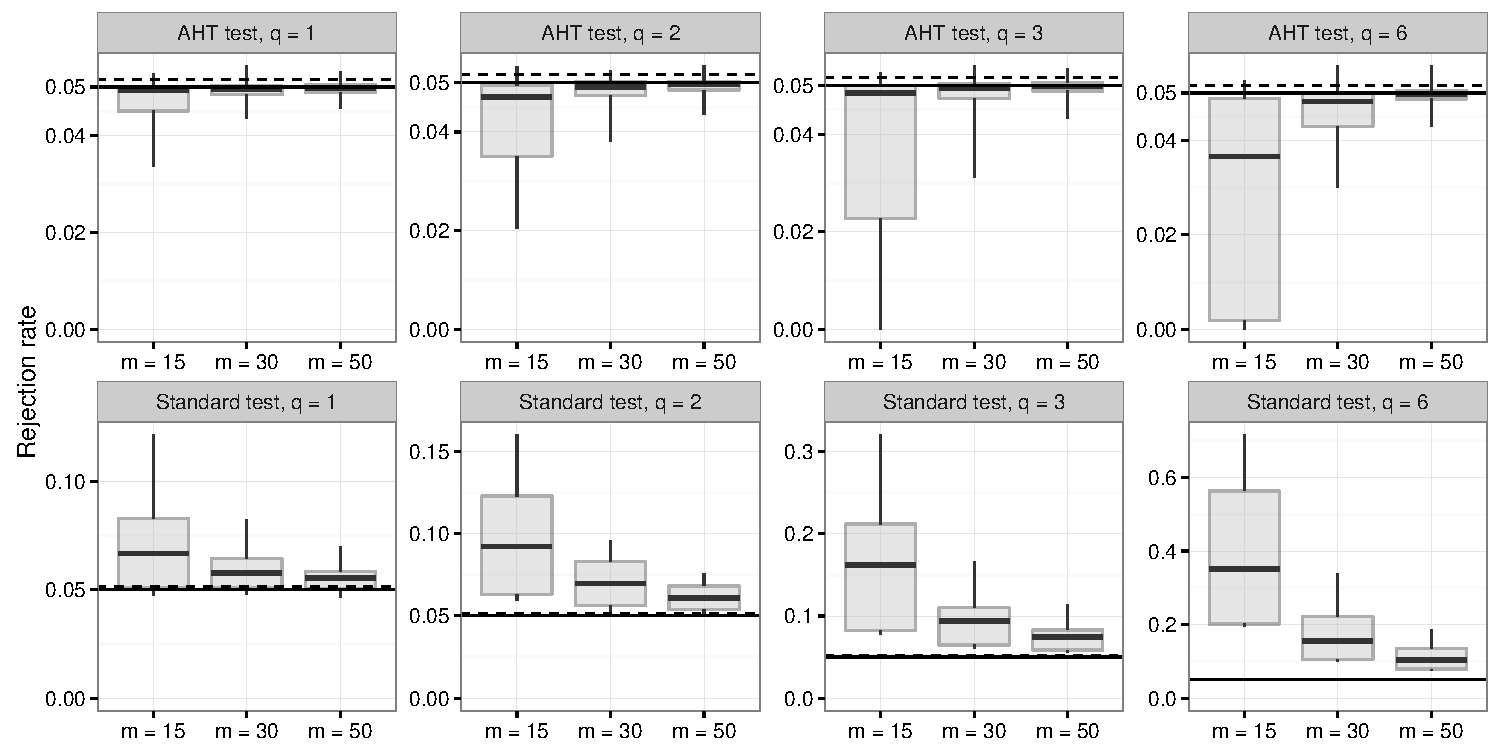
\includegraphics[width=\linewidth]{CR_fig/overview-1} 

}

\caption[Rejection rates of AHT and standard tests for ]{Rejection rates of AHT and standard tests for $\alpha = .05$, by dimension of hypothesis ($q$) and sample size ($m$). The solid horizontal line indicates the stated $\alpha$ level and the dashed line indicates an upper confidence bound on simulation error.}\label{fig:overview}
\end{sidewaysfigure}


\end{knitrout}

We discuss four main findings from the simulation results.\footnote{
Throughout, we present results for the nominal Type I error rate of $\alpha = .05$; figures presenting results for $\alpha = .01$ and $\alpha = .10$ are available in the supplementary materials, along with complete numerical results and replication code.}
The first finding is that the AHT test has Type I error close to the stated $\alpha$ level for all parameter combinations studied, whereas the standard test does not. 
Figure \ref{fig:overview} illustrates this pattern at the nominal type I error rate of $\alpha = .05$, for constraints of varying dimension (from $q = 1$, in the first column, to $q = 6$, in the final column) and varying number of clusters.
It can be seen that the AHT test has Type I error near the stated $\alpha$ level, even with a small number of clusters.
When the number of clusters is very small, the Type I error can be smaller than the stated $\alpha$ level. 
Although there exist situations in which the error is above the simulation bound, the departures are typically small. For example, when $m = 15$ the rejection rates do not exceed 0.012 for $\alpha = .01$, 0.019 for $\alpha = .05$, and 0.073 for $\alpha = .10$.
The rejection rates are even closer to nominal for lower-dimensional constraints.

In comparison to the AHT test, the Type I error for the standard test can be markedly higher than the stated $\alpha$ level, particularly when the number of clusters is small or the dimension of the hypothesis is large. 
For example, the maximum Type I error ranges from 0.123 ($q = 1$) to 0.682 ($q = 6$) for data sets with 15 clusters.
Perhaps even more important for practice, the rejection rate of the standard test can be far above the stated $\alpha$ level even when there are 50 clusters, with maximum error ranging from 0.073 ($q = 1$) to 0.18 ($q = 6$).

\begin{knitrout}
\definecolor{shadecolor}{rgb}{0.969, 0.969, 0.969}\color{fgcolor}\begin{sidewaysfigure}

{\centering 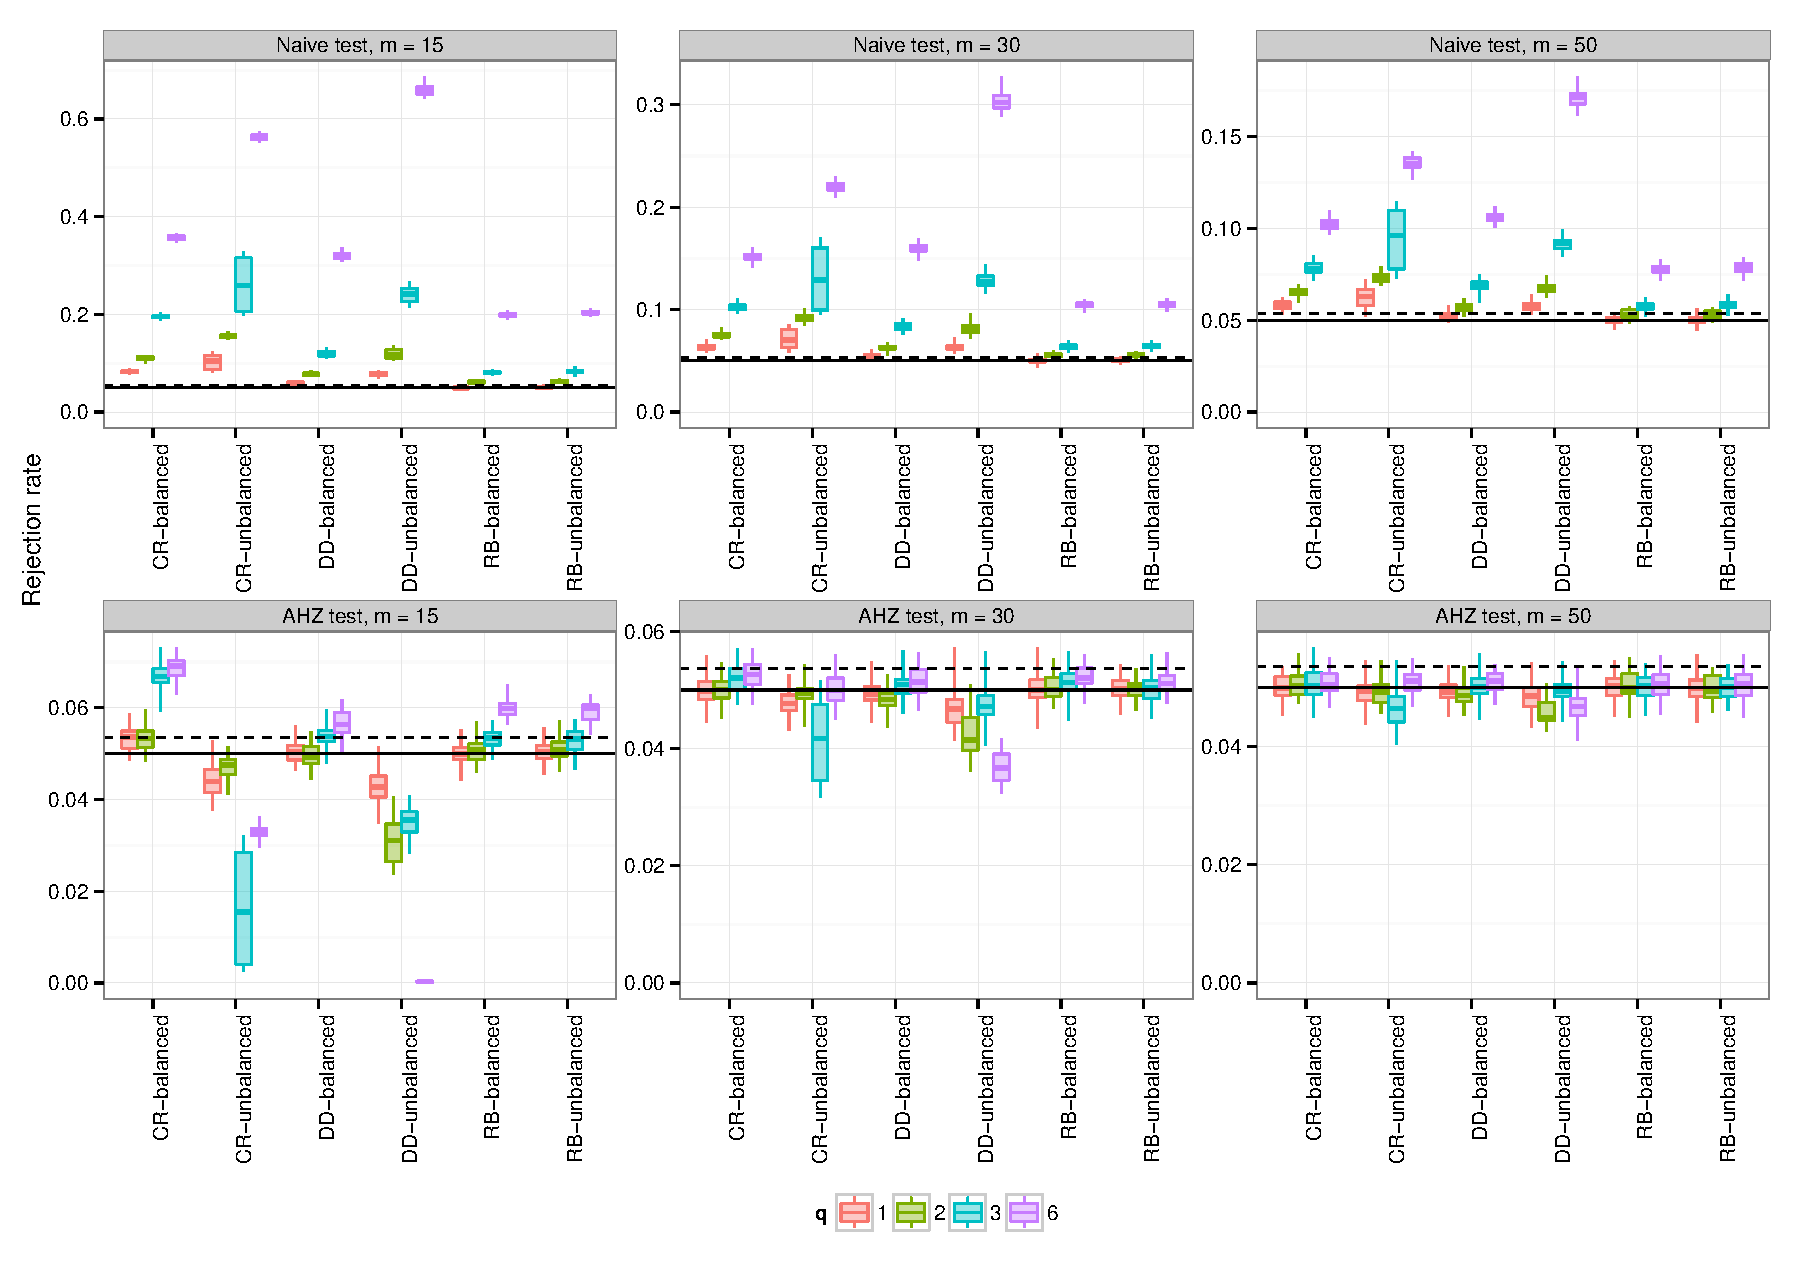
\includegraphics[width=\linewidth]{CR_fig/balance-1} 

}

\caption[Rejection rates of AHT and standard tests, by study design and dimension of hypothesis (]{Rejection rates of AHT and standard tests, by study design and dimension of hypothesis ($q$) for $\alpha = .05$ and $m = 30$. The solid horizontal line indicates the stated $\alpha$ level and the dashed line indicates an upper confidence bound on simulation error. CR = cluster-randomized design; DD = difference-in-differences design; RB = randomized block design; B = balanced; U = unbalanced.}\label{fig:balance}
\end{sidewaysfigure}


\end{knitrout}

Figure \ref{fig:balance} breaks out the rejection rates by study design, focusing on a sample size of $m = 30$. 
In the bottom panel, it can be seen that the rejection rate of the standard test increases with the dimension of the test ($q$) and the degree of unbalance in the study design.
Differences between the balanced and unbalanced designs are largest for the CR and DD designs, with smaller discrepancies in RB designs.
The top row of Figure \ref{fig:balance} displays results for the AHT test.
For studies with at least 30 clusters, rejection rates of the AHT test are very closes to nominal (between 0.031 and 0.058) across all conditions studied.
Unbalanced designs led to rejection rates that were usually below the nominal $\alpha$---just the opposite of how the standard test is affected by unbalance. 
This trend is the strongest for CR and DD designs. At the smallest sample size, the rejection rate of the AHT test could be close to 0 in unbalanced CR and DD designs (see supplementary figures S3-S5). 

By simulating the errors across a variety of parameter combinations, we were also able to test the impact of misspecification of the working model on Type I error.
Because the CR2 correction and AHT degrees of freedom are both based on a working model with independent, homoskedastic errors, model misspecification increases with the true level of treatment effect variance ($\sigma_\delta^2$) and intra-class correlation ($\tau^2$).
Across the nine error structures, the range of rejection rates remains very similar for the AHT test, with no clear pattern related to the degree of mis-specification (see supplementary figures S11-S13). 
These findings follow closely those from \maskcitet{Tipton2015small-F}, which also found that the Type I error of the AHT test was close to nominal even when the working model was very discrepant from the data-generating model.

\begin{knitrout}
\definecolor{shadecolor}{rgb}{0.969, 0.969, 0.969}\color{fgcolor}\begin{figure}

{\centering 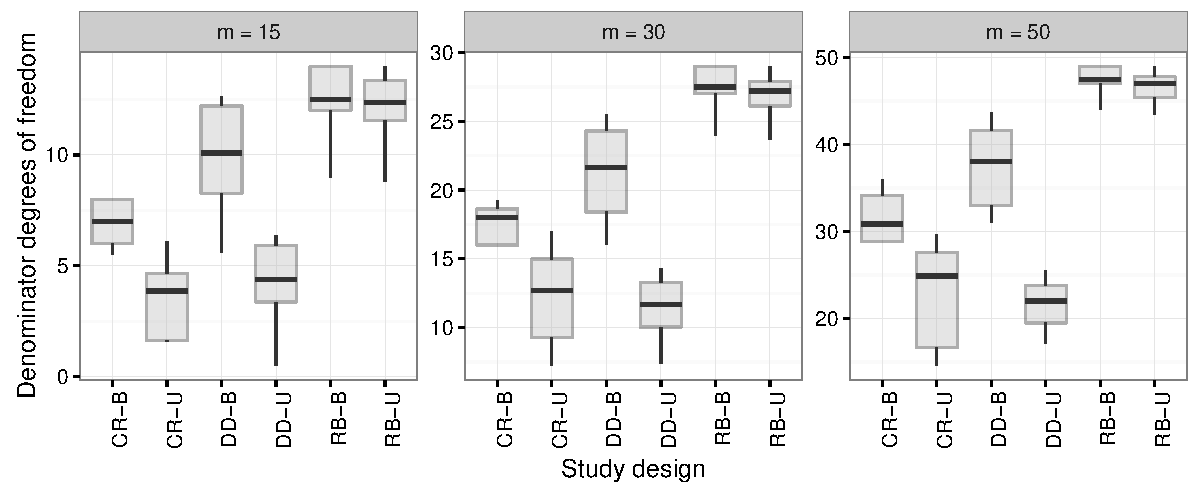
\includegraphics[width=\linewidth]{CR_fig/df-1} 

}

\caption[Range of denominator degrees of freedom for AHT test, by number of clusters and study design]{Range of denominator degrees of freedom for AHT test, by number of clusters and study design. CR = cluster-randomized design; DD = difference-in-differences design; RB = randomized block design; B = balanced; U = unbalanced.}\label{fig:df}
\end{figure}


\end{knitrout}

Finally, Figure \ref{fig:df} depicts the range of estimated degrees of freedom for the AHT test as a function of the simulated study design and number of clusters ($m$). 
Within each box plot, the degrees of freedom vary depending on the hypothesis tested, with constraints of larger dimension having lower degrees of freedom. 
It can be seen that the AHT degrees of freedom are often far less than $m - 1$ and that they are strongly affected by the pattern of treatment assignment and the degree of balance. The balanced and unbalanced RB designs generally had AHT degrees of freedom closest to $m - 1$ because the treatment effects being tested are all identified within each cluster. 
The balanced DD design usually had the next largest degrees of freedom because it involved contrasts between two patterns of treatment configuration, followed by the balanced CR design, which involved contrasts between three patterns of treatment configurations. 
For both of these designs, unbalance led to sharply reduced degrees of freedom.

In summary, these results demonstrate that the standard robust Wald test, using the CR1 correction and $m - 1$ degrees of freedom, produces a wide range of rejection rates, often far in excess of the nominal Type I error. 
In contrast, the rejection rates of the AHT test are below or at most slightly above nominal, across all of the conditions examined.
This is because the AHT test incorporates information about the covariate features into its estimated degrees of freedom, whereas the standard test does not.
An important question that remains then is how much the AHT and standard tests diverge in actual application.
%In the next section, we compare the two tests in several examples drawn from recent empirical research.

\section{EXAMPLES}
\label{sec:examples}

This section presents two examples that illustrate the performance of CRVE in different applied contexts. 
In the first example, the effects of substantive interest involve between-cluster contrasts. 
The second example involves a cluster-robust Hausman test for differences between within- and across-cluster information. 
In each example, we demonstrate the proposed AHT test for single- and multiple-parameter hypotheses and compare the results to the standard test based on the CR1 variance estimator and $m - 1$ degrees of freedom. 
The focus here is on providing insight into the conditions under which the AHT and standard estimators diverge in terms of three quantities of interest: the standard error estimates, the degrees of freedom estimates, and the stated p-values. 
Data files and replication code are available in the supplementary materials.

\subsection{Achievement Awards demonstration} 

\citet{Angrist2009effects} reported results from a randomized trial in Israel that aimed to increase completion rates of the Bagrut, the national matriculation certificate for post-secondary education, among low-achieving high school students. 
In the Achievement Awards demonstration, 40 non-vocational high schools with low rates of Bagrut completion were selected from across Israel, including 10 Arab and 10 Jewish religious schools and 20 Jewish secular schools. 
The schools were then pair-matched based on 1999 rates of Bagrut completion, and within each pair one school was randomized to receive a cash-transfer program. 
In these treatment schools, seniors who completed certification were eligible for payments of approximately \$1,500. 
Student-level covariate and outcome data were drawn from administrative records for the school years ending in June of 2000, 2001, and 2002. 
The incentive program was in effect for the group of seniors in treatment schools taking the Bagrut exams in Spring of 2001, but the program was discontinued for the following year. 
We therefore treat completion rates for 2000 and 2002 as being unaffected by treatment assignment.
The primary outcome of interest is Bagrut completion. 

This study provides an opportunity to examine the AHT test in a study with relatively few clusters, with treatment assigned at the cluster level.
For simplicity, we restrict our analysis to the sample of female students, which reduces the total sample to 35 schools.
Following the original analysis of \citet{Angrist2009effects}, we allow the program's effects to vary depending on whether a students was in the upper or lower half of the distribution of prior-year academic performance. 
Letting $h = 1,2,3$ index the sector of each school (Arab religious, Jewish religious, or Jewish secular), we consider the following analytic model: 
\begin{equation}
\label{eq:AL_ATE}
y_{hitj} = z_{hit}\bm{r}_{hitj}'\bs\beta_h + \bm{s}_{hitj}'\bs\gamma + \gamma_{ht} + \mu_{hi} + \epsilon_{hitj}
\end{equation}
In this model for student $j$ in year $t$ in school $i$ in sector $h$, $z_{hit}$ is an indicator equal to one in the treatment schools for the 2001 school year and otherwise equal to zero; $\bm{r}_{hitj}$ is a vector of indicators for whether the student is in the lower or upper half of the distribution of prior academic performance; and $\bs\beta_h = \left(\beta_{1h}, \beta_{2h}\right)$ is a vector of average treatment effects for schools in sector $h$. 
The vector $\bm{s}_{hitj}$ includes the following individual student demographic measures: mother's and father's education, immigration status, number of siblings, and indicators for each quartile in the distribution of prior-year academic performance. 
The model also includes fixed effects $\gamma_{ht}$ for each sector in each year and $\mu_{hi}$ for each school. 

Based on Model (\ref{eq:AL_ATE}), we test four hypotheses.%, again with the goal of exploring the use of the AHT tests under a range of conditions. 
First, we assume that the program effects are constant across sector (i.e., $\bs\beta_1 = \bs\beta_2 = \bs\beta_3 = \bs\beta$) and test for whether the program affected completion rates for students in the upper half of the prior achievement distribution ($H_0: \beta_2 = 0$, with $q = 1$).
Second, we test for whether the program was effective in either half of the prior academic performance ($H_0: \bs\beta = 0$, with $q = 2$), still assuming that program effects are constant across sector. 
Third, we test for whether program effects in the upper half of the prior achievement distribution are moderated by school sector ($H_0: \beta_{21} = \beta_{22} = \beta_{23}$, with $q = 3$). 
Finally, we conduct a joint test for whether program effects in either half of the prior achievement distribution are moderated by school sector ($H_0: \bs\beta_1 = \bs\beta_2 = \bs\beta_3$, with $q = 4$). 



% latex table generated in R 3.2.5 by xtable 1.7-4 package
% Mon Jul 04 21:58:33 2016
\begin{table}[bth]
\centering
\caption{Tests of treatment effects in the Achievement Awards Demonstration} 
\label{tab:AAD}
\begin{tabular}{lcrrr}
  \toprule
Hypothesis & Test & F & df & p \\ 
  \midrule
ATE - upper half (q = 1) & Standard & 5.746 & 34.00 & 0.02217 \\ 
   & AHT & 5.169 & 15.86 & 0.03726 \\ 
  ATE - joint (q = 2) & Standard & 3.848 & 34.00 & 0.03116 \\ 
   & AHT & 3.371 & 15.46 & 0.06096 \\ 
   \midrule
Moderation - upper half (q = 2) & Standard & 3.186 & 34.00 & 0.05393 \\ 
   & AHT & 0.091 & 3.19 & 0.91520 \\ 
  Moderation - joint (q = 4) & Standard & 8.213 & 34.00 & 0.00010 \\ 
   & AHT & 2.895 & 3.21 & 0.19446 \\ 
   \bottomrule
\end{tabular}
\end{table}


Table \ref{tab:AAD} reports the results of all four hypothesis tests. 
For the first two hypotheses, the AHT test statistics are slightly smaller than their standard counterparts and the degrees of freedom are considerably smaller. 
These differences in degrees of freedom arise because the treatment was assigned at the cluster level, while the subgroups varied within each cluster. 
In contrast, the AHT and standard tests diverge markedly for the third and fourth hypotheses tests, which compared treatment effects across sectors and subgroups.
For these cases, the AHT test statistic and degrees of freedom are both considerably smaller than those from the standard test. 
This reflects the degree of unbalance in allocations across sectors (19 Jewish secular, 7 Jewish religious, and 9 Arab religious schools), combined with cluster-level randomization. 
In combination, these smaller test statistics and degrees of freedom result in larger p-values for the AHT test when compared to the standard test.

\subsection{Effects of minimum legal drinking age on mortality} 

As a second illustration, we draw on a panel data analysis described in \citet[see also \citealp{Carpenter2011minimum}]{Angrist2014mastering}.
Based on data from the Fatal Accident Reporting System maintained by the National Highway Traffic Safety Administration, we estimate the effects of changes in the minimum legal drinking age over the time period of 1970-1983 on state-level death rates resulting from motor vehicle crashes.
A standard difference-in-differences specification for such a state-by-year panel is
\begin{equation}
\label{eq:MLDA}
y_{it} = \bm{r}_{it}'\bs\beta + \gamma_t + \mu_i + \epsilon_{it}.
\end{equation}
In this model, time-point $t$ is nested within state $i$; the outcome $y_{it}$ is the number of deaths in motor vehicle crashes (per 100,000 residents) in state $i$ at time $t$; $\bm{r}_{it}$ is a vector of covariates; $\gamma_t$ is a fixed effect for time point $t$; and $\mu_i$ is an effect for state $i$. The vector $\bm{r}_{it}$ consists of a measure of the proportion of the population between the ages of 18 and 20 years who can legally drink alcohol and a measure of the beer taxation rate, both of which vary across states and across time.\todo{Possible to get replication data from Carpenter and Dobkin (2011) instead?}

We apply both random effects (RE) and fixed effects (FE) approaches to estimate the effect of lowering the legal drinking age. 
For the RE estimates, we use feasible GLS based the assumption that  $\mu_1,...,\mu_m$ are mutually independent, normally distributed, and independent of $\epsilon_{it}$ and $\bm{r}_{it}$.
We also report an artificial Hausman test \citep{Arellano1993on, Wooldridge2010econometric} for correlation between the covariates $\bm{r}_{it}$ and the state effects $\mu_i$. Such correlation creates bias in the RE estimator of the policy effect, thus necessitating the use of the FE estimator.
The artificial Hausman test amends model (\ref{eq:MLDA}) to include within-cluster deviations for the variables of interest, so that the estimating equation is
\begin{equation}
y_{it} = \bm{r}_{it}\bs\beta + \bm{\ddot{r}}_{it}\bs\delta + \gamma_t + \mu_i + \epsilon_{it},
\end{equation}
where $\bm{\ddot{r}}_{it}$ denotes the within-cluster deviations of the covariate.
The parameter $\bs\delta$ captures the difference between the between-cluster and within-cluster estimates of $\bs\beta$. 
With this setup, the artificial Hausman test amounts to testing the null hypothesis that $\bs\delta = \bm{0}$, where $\bs\delta$ is estimated using RE.  



% latex table generated in R 3.2.5 by xtable 1.7-4 package
% Mon Jul 04 21:58:33 2016
\begin{table}[bth]
\centering
\caption{Tests of effects of minimum legal drink age and Hausman specification test} 
\label{tab:MLDA}
\begin{tabular}{lcrrr}
  \toprule
Hypothesis & Test & F & df & p \\ 
  \midrule
Random effects & Standard & 8.261 & 49.00 & 0.00598 \\ 
   & AHT & 7.785 & 24.74 & 0.00999 \\ 
  Fixed effects & Standard & 9.660 & 49.00 & 0.00313 \\ 
   & AHT & 9.116 & 22.72 & 0.00616 \\ 
   \midrule
Hausman test & Standard & 2.930 & 49.00 & 0.06283 \\ 
   & AHT & 2.489 & 8.69 & 0.13980 \\ 
   \bottomrule
\end{tabular}
\end{table}


Table \ref{tab:MLDA} displays the results of the tests for the policy variable and the Hausman tests for each model specification. 
The results of the policy effect tests are quite similar across specifications and versions of the test. 
Of note is that, for both the RE and FE estimates, the AHT tests have only half the degrees of freedom of the corresponding standard tests. 
For the artificial Hausman test, the AHT test has fewer than 9 degrees of freedom, which leads to a much larger p-value compared to using the standard test based on CR1. 

\section{Conclusion}
\label{sec:conclusion}

Empirical studies in economics often involve modeling data with a correlated error structure. 
%Correlated errors arise in the analysis of multi-stage samples, cluster-randomized trials, panel data, and regression discontinuities with discrete forcing variables, among other study designs. 
It is now routine to handle dependent error structures by using cluster-robust variance estimation, which provides asymptotically valid standard errors and hypothesis tests without making strong parametric assumptions about the error structure. 
However, a growing body of recent work has drawn attention to the shortcomings of CRVE methods when the data include only a small or moderate number of independent clusters \citep{Cameron2008bootstrap, Cameron2015practitioners, Imbens2015robust, MacKinnon2016wild}. 
In particular, Wald tests based on CRVE can have rejection rates far in excess of the nominal Type I error. 
This problem is compounded by the fact that the performance of standard Wald tests depends on features of the study design beyond just the total number of clusters, which can make it difficult to determine whether standard, asymptotic valid CRVE methods are accurate. 

One promising solution to this problem is to use the bias-reduced linearization variance estimator (i.e., CR2) proposed by \citet{Bell2002bias}, which corrects the CRVE so that it is exactly unbiased under an analyst-specified working model for the error structure, together with degrees of freedom estimated based on the same working model.
In this paper, we have extended the CR2 variance estimator so that it is a fully general solution, which can be applied to test single- or multi-dimensional parameter constraints in models with fixed effects in multiple dimensions. 
%With the modifications and extensions proposed in this paper, the CR2 variance estimator and small-sample testing procedures can be applied in a wide range of analytic models---essentially, any model estimated by ordinary or weighted least squares. 
We join \citet{Imbens2015robust} in arguing that the CR2 estimator and corresponding estimated degrees of freedom for hypothesis tests should be applied routinely, whenever analysts use CRVE and hypothesis tests based thereon. 
Because the performance of standard CRVE methods depends on features of the study design, the total number of clusters in the data is an insufficient guide to whether small-sample corrections are needed. 
Instead, the clearest way to determine whether small-sample corrections are needed is simply to calculate them.

The proposed AHT test involves two adjustments: use of the CR2 adjustment for the variance estimator and use of estimated degrees of freedom. 
%Used in combination, the AHT test has Type I error close to the stated $\bs\alpha$ level. 
Our empirical examples illustrate that the degrees of freedom adjustment can have a relatively large influence on small-sample performance.
These degrees of freedom can be much smaller than the number of clusters, particularly when the covariates involved in the test involve high leverage or are unbalanced across clusters.
The estimated degrees of freedom are indicative of the precision of the standard errors, and thus provide diagnostic information that is similar to the effective sample size measure proposed by \citet{Carter2013asymptotic}. 
We therefore recommend that the degrees of freedom be reported along with standard errors and $p$-values whenever the method is applied.

The idea of developing small-sample adjustments based on a working model may seem strange to analysts accustomed to using CRVE---after all, the whole point of clustering standard errors is to avoid making assumptions about the error structure.
However, simulation studies reported here and elsewhere \maskcitep{Tipton2015small-t, Tipton2015small-F} have demonstrated that the approach is actually robust to a high degree of misspecification in the working model. 
Furthermore, while the working model provides necessary scaffolding when the number of clusters is small, its  influence tends to fall away as the number of clusters increases, so that the CR2 estimator and AHT maintain the same asymptotic robustness as standard CRVE methods. 

One outstanding problem with the CR2 variance estimator is that it can become computationally costly (or even infeasible) when the within-cluster sample sizes are large \citep{Mackinnon2015wildCIs}. 
For example, \citet{Bertrand2004how} analyzed micro-level data from a 21-year panel of current population survey data, with clustering by state. Their data included some state-level clusters with over $n_i = 10,000$ individual observations. 
The CR2 adjustment matrices have dimension $n_i \times n_i$, and would be very expensive to compute in this application. 
Methods for improving the computational efficiency of the CR2 variance estimator (or alternative estimators that have similar performance to CR2), should be investigated further. 

This paper has developed the CR2 estimator and AHT testing procedure for weighted least squares estimation of linear regression models. 
Extensions to linear regression models with clustering in multiple, non-nested dimensions \citep[cf.][]{Cameron2011robust} appear to be possible, and their utility should be further investigated. 
\citet{McCaffrey2006improved} have proposed extensions to bias-reduced linearization for use with generalized estimating equations, and future work should consider further extensions to other classes of estimators, including two-stage least squares and generalized method of moments. 

\bibliographystyle{agsm}
\bibliography{bibliography}

\end{document}

